% DASA'26 draft — Track 2: Engineering Decision Making in Healthcare
% IEEE conference format, 5-page limit. Compile: pdflatex main; bibtex main; pdflatex main x2
% All numbers are taken from results/ (see paper/NUMBERS.md for the source of each).
\documentclass[conference]{IEEEtran}
\IEEEoverridecommandlockouts
\usepackage{cite}
\usepackage{amsmath,amssymb}
\usepackage{graphicx}
\usepackage{booktabs}
\usepackage{multirow}
\usepackage[hidelinks]{hyperref}
\usepackage{xcolor}
\newcommand{\todo}[1]{\textcolor{red}{[TODO: #1]}}

\begin{document}

\title{When Is Imperfect Triage Better Than None?\\
Load-Dependent Break-Even Accuracy for ML Triage\\ in Emergency Priority Queues}

\author{\IEEEauthorblockN{Tanishq Singh Sisodiya}
\IEEEauthorblockA{\todo{Department, Institution}\\
\todo{City, Country}\\
sisodiya.tanishq.singh@gmail.com}}

\maketitle

\begin{abstract}
Hospitals considering machine-learning (ML) triage need a minimum quality bar:
how good must an acuity classifier be before prioritising patients by its output
serves high-acuity patients better than first-in-first-out (FIFO)? We show that the
answer depends on the metric. For mean waiting time the break-even is Youden's
$J=0$ at every load, a direct consequence of priority-queue algebra. For the
95th-percentile wait of high-acuity patients, a validated discrete-event simulation
of a five-level multi-server emergency department (ED) gives a bar that rises
with utilisation: no break-even exists up to $\rho=0.7$, and the required high-acuity
Youden $J$ grows from 0.13 at $\rho=0.8$ to 0.24 at $\rho=0.95$. An accumulating
priority queue (APQ) lowers the bar at every load. Target compliance, often
used in practice, is unsuitable as a sole criterion: even an almost uninformative
classifier improves it. Using 108,180 visits from the U.S.\ NHAMCS survey and an
outcome-based reference acuity, we place a nurse-triage and a LightGBM operating point
on the map. Both clear the tail bar by a wide margin, because real triage errors are
mostly off by one level; the fraction of high-acuity patients sent to the two lowest
levels (4\% nurse, 12\% ML) is far below the break-even of about 30\%. The operating
points differ mainly in the harm they impose on low-acuity patients, which APQ
more than halves. The results give ED managers a load-indexed lookup of classifier
quality and policy.
\end{abstract}

\begin{IEEEkeywords}
emergency department, triage, priority queues, machine learning, discrete-event simulation,
decision support
\end{IEEEkeywords}

% ============================================================================
\section{Introduction}

Emergency departments (EDs) prioritise patients by an acuity level assigned at triage,
usually on a five-level scale such as the Emergency Severity Index or the Canadian
Triage and Acuity Scale (CTAS)~\cite{bullard2017ctas}. Nurse triage is itself imperfect:
a systematic review reports substantial under- and over-triage~\cite{hinson2019triage}.
ML classifiers trained on triage-time data are an appealing supplement, but a decision
maker needs to know how accurate such a classifier must be, at the ED's operating
load, before priority by its predictions beats simply seeing patients in arrival
order, and how it compares with the nurses it would assist.

Priority assignment under imperfect class information is not new. Argon and
Ziya~\cite{argon2009priority} study two-type queues in which each customer carries a
noisy signal of its type; Sun, Argon and Ziya ask when error-prone triage is worth
doing at all~\cite{sun2022triage,sun2018austere}; feature-driven priority queuing trains
the classifier to minimise waiting cost~\cite{fdpq2024}; and the accumulating priority
queue (APQ) was designed for EDs with acuity-specific time
targets~\cite{stanford2014apq}. Our contribution is narrower and empirical:
\begin{enumerate}
\item A short observation that the two-class mean-wait break-even is $J=0$ at every
load, which explains why mean wait is the wrong yardstick (Section~\ref{sec:prop}).
\item Load-dependent break-even surfaces for tail waits of high-acuity patients under a
five-level ordinal error model with separate noise and bias, for strict priority and
APQ, from a simulator validated against closed-form results (Sections~\ref{sec:model}--\ref{sec:surfaces}).
\item Nurse and ML operating points, both scored against the same outcome-based
reference acuity on public NHAMCS data, placed on the map, with a queue-aware
threshold choice for the ML model (Section~\ref{sec:real}).
\item Two cautions for practitioners: target compliance can be improved by an
uninformative classifier, and high-acuity Youden $J$ does not predict queue impact
for real classifiers, whereas the rate of \emph{severe} undertriage does.
\end{enumerate}

% ============================================================================
\section{Model and Methods}\label{sec:model}

\subsection{Queue, classifier and policies}
Patients arrive as a Poisson process; each has a true acuity level $k\in\{1,\dots,5\}$
(1 most urgent) drawn i.i.d.\ from a mix $\pi$ and receives exponential service with
mean 20~min from one of $c$ identical providers ($c=5$ for the main results, $c=1$ for
analytic checks). Utilisation is $\rho=\lambda\,\mathbb{E}[S]/c\in\{0.5,\dots,0.95\}$.
The predicted level follows an ordered-probit error model with noise $\sigma$ and bias $b$:
\begin{equation}
\hat k=\min\{5,\max\{1,\operatorname{round}(k+b+\sigma\varepsilon)\}\},\quad
\varepsilon\sim\mathcal N(0,1),
\end{equation}
where $b>0$ is systematic undertriage. Each $(\sigma,b)$ yields a closed-form $5\times5$
confusion matrix, from which we report interpretable quantities: high-acuity
(levels 1--2 vs.\ 3--5) sensitivity, specificity and Youden $J$, and
\emph{severe undertriage} $\mathrm{SU}=P(\hat k\ge4\mid k\le2)$. The simulator also
accepts any empirical confusion matrix (plug-in mode).
Policies are FIFO; non-preemptive priority by predicted level (NP-PQ, FIFO within a level);
an oracle NP-PQ on true levels; and APQ, in which a waiting patient accrues priority
$w_{\hat k}\cdot(\text{time waited})$ with $w=(16,8,4,2,1)$~\cite{kleinrock1964delay,stanford2014apq}.

\subsection{Metrics}
Time-to-provider targets are $\tau=(5,15,30,60,120)$~min, modelled on
CTAS~\cite{bullard2017ctas}. For true levels 1--2 we record target compliance
$\mathrm{TC}_{12}=P(W\le\tau_k)$, mean wait, and the 90th/95th percentiles
(p90$_{12}$, p95$_{12}$); the cost to low-acuity patients is the p95 wait of levels 4--5
(p95$_{45}$). The primary endpoint is p95$_{12}$, for reasons shown in
Section~\ref{sec:two}.

\subsection{Mean-wait break-even is load-independent}\label{sec:prop}
Consider two classes (H, L), NP-PQ on the predicted class, M/G/1 with loads
$\rho_H,\rho_L$, $\rho=\rho_H+\rho_L<1$, mean residual work $W_0$, sensitivity $s$ and
specificity $p$. By Cobham's formula~\cite{cobham1954priority} a predicted-high patient
waits $W_0/(1-\sigma_1)$ and a predicted-low one $W_0/[(1-\sigma_1)(1-\rho)]$, where
$\sigma_1=s\rho_H+(1-p)\rho_L$ is the predicted-high load; FIFO gives $W_0/(1-\rho)$. Hence
\begin{equation}
\overline W_H^{\text{triage}}<\overline W^{\text{FIFO}}\iff 1-s\rho<1-\sigma_1
\iff s+p>1 .
\end{equation}
The break-even is $J=s+p-1=0$, independent of $\rho$, the class mix and the service
distribution; for M/M/$c$ with a common rate the Erlang-C factor cancels the same way.
This follows from standard results~\cite{cobham1954priority,kleinrock1965conservation}
and is closely related to~\cite{argon2009priority}; we use it only to motivate tail
metrics. The same algebra gives exact five-level mean waits under any confusion matrix,
which we use to check the simulator.

\subsection{Simulation, validation and break-even estimation}
A SimPy reference simulator and a Numba event-loop kernel (250,000 patients in about
15~ms) give identical per-patient waits on common inputs. Each replication uses 100,000
patients (250,000 for $\rho\ge0.9$), discards a 10\% warm-up (checked with Welch's
method at $\rho=0.95$~\cite{welch1983}), and pre-draws arrivals, service times, true
levels and the noise $\varepsilon$ once; the same draws are reused for every policy and
every $(\sigma,b)$ (common random numbers~\cite{law2015simulation}). Validation against
closed forms ran on the SimPy engine with 30 replications at $\rho\in\{0.5,0.7,0.9\}$
(Table~\ref{tab:val}): M/M/1 and M/G/1 FIFO (Pollaczek--Khinchine), five-level M/G/1
NP-PQ (Cobham), M/M/5 NP-PQ, the conservation law~\cite{kleinrock1965conservation},
two-class misclassified NP-PQ, and two- and five-class APQ
(Kleinrock's delay-dependent recursion~\cite{kleinrock1964delay}). All 81 mean waits
are within 1.4\% of the analytic value; 80 of the 81 95\% intervals cover it, and the
two flagged checks are consistent with chance. Across all 2,380 five-level NP-PQ sweep
cells, simulated mean waits of levels 1--2 match the analytic mixture formula with a
median error of 0.55\% (95th percentile 1.7\%).

The main sweep crosses $\sigma\in\{0,0.1,\dots,2\}\cup\{2.25,\dots,20\}$ (34 values),
$b\in\{0,\pm0.25,\pm0.5\}$, seven loads, $c\in\{1,5\}$ and two policies, with 20
replications per cell. For each cell we form paired replication differences
$\Delta(\sigma)$ against FIFO, locate the sign change by linear interpolation to obtain
$\sigma^*$, bootstrap the replications (1,000 resamples) for a 95\% interval, and convert
$\sigma^*$ to $J^*$ and $\mathrm{SU}^*$ with the closed-form confusion matrix. The grid
extends beyond $\sigma=2$ because at $\sigma=2$ the high-acuity $J$ is still 0.36.

\begin{table}[t]
\caption{Simulator validation (SimPy engine, 30 replications, $\rho\in\{0.5,0.7,0.9\}$).}
\label{tab:val}
\centering\footnotesize
\begin{tabular}{@{}llrc@{}}
\toprule
ID & Case (analytic reference) & max $|\text{err}|$ & CI covers \\
\midrule
V1 & M/M/1 FIFO & 0.63\% & 2/3 \\
V2 & M/G/1 FIFO, lognormal CV 1.5 (P--K) & 0.37\% & 3/3 \\
V3 & M/G/1 NP-PQ, 5 levels (Cobham) & 0.79\% & 15/15 \\
V4 & M/M/5 NP-PQ, 5 levels & 0.64\% & 15/15 \\
V5 & Conservation law, FIFO/NP-PQ/APQ & 0.15\% & 9/9 \\
V6 & 2-class misclassified NP-PQ & 1.36\% & 15/15 \\
V7 & APQ, 2 and 5 classes (Kleinrock) & 1.07\% & 21/21 \\
V8 & Confusion sampling, $10^6$ draws/row & $\le$0.0014 & 10/10 \\
\bottomrule
\end{tabular}
\\[2pt]\raggedright\scriptsize V8 reports max.\ absolute difference in probability.
V6 also checks the sign of the paired difference against FIFO at $J\in\{-0.3,0,0.3,0.7\}$;
the one miss is a +0.19~min difference at $J=0$, $\rho=0.7$ (on a 47-min wait).
\end{table}

\subsection{Data, reference acuity and classifiers}\label{sec:data}
We use the NHAMCS ED public-use files for 2016--2019 and 2021--2022 (108,180
visits)~\cite{nhamcs}. The reference acuity (rESI-O) is built only from post-triage
outcomes and resources, frozen before training: level 1 for death in the ED, CPR,
intubation or BiPAP/CPAP; level 2 for admission to critical care, operating room or
catheterisation lab, or in-hospital death; level 3 for any other admission or transfer,
or at least two ESI-type resources (labs, ECG, X-ray, advanced imaging, IV fluids,
nebulised medication, consultation, procedures); levels 4 and 5 for one and zero resources.
Visits that arrived dead or left before care was complete were excluded (3,336); 99.2\%
of the remaining 104,844 received a label. The survey-weighted mix
$\pi=(0.009,0.027,0.489,0.233,0.242)$ is used in all simulations.
The nurse operating point is the recorded immediacy level (IMMEDR), available for 69\%
of labelled visits.

Features are triage-time only: age, sex, ambulance arrival, transfer, arrival time,
initial vital signs with missing flags, pain score, 72-hour revisit, nursing-home
residence, injury flag and the 100 most frequent reason-for-visit groups (131 features);
a leakage test rejects any label-source variable. We split by time: training 2016--2018
(54,489), validation 2019 (18,812), test 2021--2022 (30,675). We fit multinomial logistic
regression (C by 5-fold GroupKFold over hospitals), LightGBM multiclass~\cite{ke2017lightgbm}
and an ordinal LightGBM regression, each LightGBM tuned by a 40-configuration random
search on validation QWK, with balanced class weights removed afterwards by prior
correction. The ML operating point maps the expected-level score to five levels with
cut-points tuned on validation QWK; shifting all cut-points by $\delta$ traces an
operating curve from overtriage ($\delta<0$) to undertriage ($\delta>0$). Confusion
matrices on the test years enter the simulator in plug-in mode.

% ============================================================================
\section{Results}

\subsection{Two classes: the metric decides the answer}\label{sec:two}
Fig.~\ref{fig:two} sweeps sensitivity $s=p$ for 20\% high-acuity patients, $c=1$.
Mean-wait curves for all loads cross zero at $J=0$ (estimated $|J^*|\le0.01$), matching
the analytic curves. The p95 wait, in contrast, has a break-even that rises from
$J^*=0.06$ at $\rho=0.5$ to 0.26 at $\rho=0.8$ and 0.35 at $\rho=0.95$: a mis-triaged
high-acuity patient queues behind all correctly placed work, and at high load that tail
dominates. Target compliance never crosses: even at $J=-0.4$ triage raises
$P(W\le\tau_H)$ by 0.004--0.024. With a target that is short relative to service time,
compliance counts only the patients lucky enough to land in the fast lane, and any
priority lottery creates such a lane.

\begin{figure*}[t]
\centering
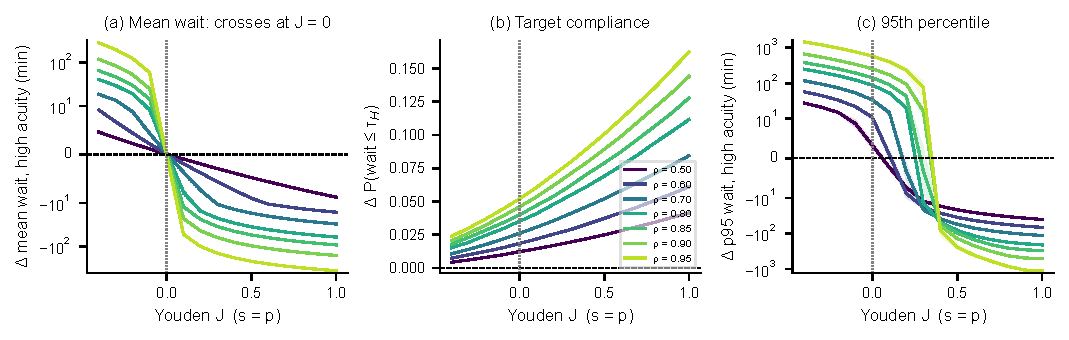
\includegraphics[width=\textwidth]{figures/F2_two_class_breakeven.pdf}
\caption{Two classes, $c=1$, 20\% high acuity: change (triage $-$ FIFO) for true
high-acuity patients vs.\ Youden $J$ along $s=p$, one line per load (dotted: analytic
mean wait; bands: 95\% CI). (a) Mean wait crosses at $J=0$ for every $\rho$; (b) target
compliance improves even for $J<0$; (c) the p95 break-even moves right as load rises.}
\label{fig:two}
\end{figure*}

\subsection{Five levels: load-dependent break-even surfaces}\label{sec:surfaces}
With five levels and $c=5$ (Fig.~\ref{fig:surface}, Table~\ref{tab:lookup}), the same
pattern appears. For p95$_{12}$, triage beats FIFO over the whole grid, down to
$J=0.04$, for $\rho\le0.7$. From $\rho=0.8$ the bar rises steadily: under NP-PQ with
unbiased errors $J^*=0.128$ [0.116, 0.138] at $\rho=0.8$ and 0.236 [0.227, 0.246] at
$\rho=0.95$. In severe-undertriage terms, triage beats FIFO while
$\mathrm{SU}<\mathrm{SU}^*$, and $\mathrm{SU}^*$ falls from 0.39 to 0.30 across the same loads.
APQ lowers the bar at every load ($J^*=0.193$ at $\rho=0.95$). Bias matters less than
anticipated: moving from $b=-0.5$ to $b=+0.5$ raises $J^*$ at $\rho=0.95$ only from 0.221
to 0.245. The p90 bar behaves similarly but starts later ($\rho\ge0.85$). Mean wait of
levels 1--2 is better than FIFO everywhere except three $\rho=0.5$ cells at the edge of the
grid ($\sigma\approx20$, $J\approx0.04$), and TC$_{12}$ never crosses: at $\sigma=20$
($J=0.04$) NP-PQ still raises TC$_{12}$ by 0.29 over FIFO at $\rho=0.95$.

The bars are robust: at $\rho=0.9$, $c=5$, NP-PQ, $J^*$ ranges from 0.190 to 0.214 across
level-dependent service times, lognormal service (CV 1.5), an acuity mix taken from nurse
labels instead of rESI-O, and a flatter APQ weight set. Changing the mean service time to
10 or 40~min leaves $J^*$ unchanged, as expected, since it only rescales time.

\begin{figure*}[t]
\centering
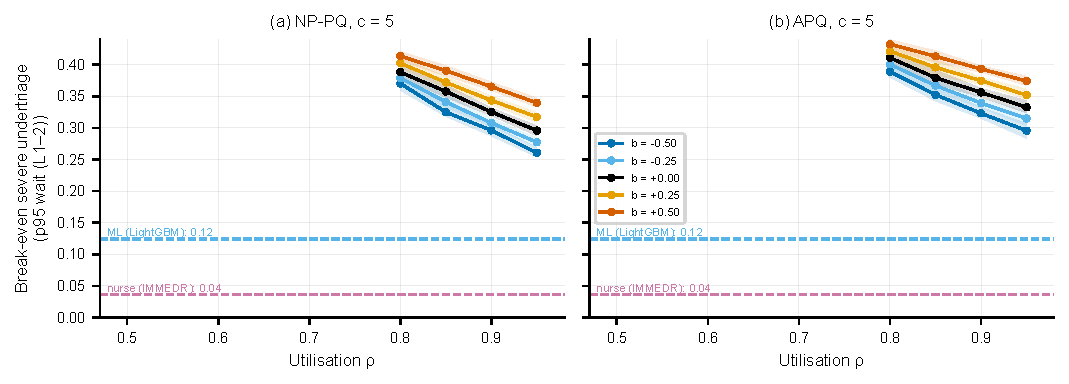
\includegraphics[width=\textwidth]{figures/F3_breakeven_p95_12_c5_severe_under_12.pdf}
\caption{Break-even severe undertriage $\mathrm{SU}^*=P(\hat k\ge4\mid k\le2)$ for the p95
wait of true levels 1--2, $c=5$, one line per bias $b$ (bands: bootstrap 95\% CI).
Below a line, triage beats FIFO; for $\rho\le0.7$ triage beats FIFO over the whole grid.
Dashed: nurse and ML operating points on the 2021--2022 test years.}
\label{fig:surface}
\end{figure*}

\begin{table}[t]
\caption{Decision lookup, $c=5$: p95$_{12}$ break-even ($b=0$) and simulated effect of the
real operating points under NP-PQ ($\Delta$ vs.\ FIFO, min; 20 replications).}
\label{tab:lookup}
\centering\footnotesize
\setlength{\tabcolsep}{3pt}
\resizebox{\columnwidth}{!}{%
\begin{tabular}{@{}lccccrrrr@{}}
\toprule
& FIFO & \multicolumn{2}{c}{$J^*$} & $\mathrm{SU}^*$ & \multicolumn{2}{c}{$\Delta$p95$_{12}$} & \multicolumn{2}{c}{$\Delta$p95$_{45}$} \\
\cmidrule(lr){3-4}\cmidrule(lr){6-7}\cmidrule(l){8-9}
$\rho$ & p95$_{12}$ & NP-PQ & APQ & NP-PQ & Nurse & ML & Nurse & ML \\
\midrule
0.50 & 7.8 & -- & -- & -- & $-2.8$ & $-2.6$ & $-0.1$ & $0.0$ \\
0.60 & 15.4 & -- & -- & -- & $-6.4$ & $-6.1$ & $+2.0$ & $+2.3$ \\
0.70 & 26.9 & -- & -- & -- & $-13.6$ & $-12.9$ & $+9.0$ & $+9.7$ \\
0.80 & 47.8 & 0.128 & 0.102 & 0.388 & $-28.7$ & $-27.9$ & $+31.2$ & $+32.5$ \\
0.85 & 68.9 & 0.163 & 0.138 & 0.357 & $-45.8$ & $-44.6$ & $+56.2$ & $+62.5$ \\
0.90 & 109.4 & 0.201 & 0.165 & 0.325 & $-81.7$ & $-80.2$ & $+103.3$ & $+144.4$ \\
0.95 & 236.6 & 0.236 & 0.193 & 0.296 & $-201.4$ & $-197.5$ & $+203.8$ & $+446.5$ \\
\bottomrule
\end{tabular}}
\\[2pt]\raggedright\scriptsize ``--'': triage beats FIFO for every classifier on the grid.
Operating points: nurse $J=0.42$, $\mathrm{SU}=0.04$; ML $J=0.21$, $\mathrm{SU}=0.12$
(at the population mix $\pi$). All $\Delta$p95$_{12}$ 95\% CIs exclude zero.
\end{table}

\subsection{Nurse and ML operating points}\label{sec:real}
Table~\ref{tab:clf} scores all operating points against rESI-O on the test years.
LightGBM ranks high-acuity patients better than nurse triage (AUROC 0.81 vs.\ 0.76) and
agrees better overall (QWK 0.54 vs.\ 0.42). Its QWK-tuned cut-points, however, rarely
assign levels 1--2, which make up only 3.6\% of visits, so its high-acuity sensitivity is
0.29 against the nurses' 0.57, and its Youden $J$ (0.21) is half the nurses' (0.42).
Accuracy-maximising argmax prediction is the extreme case: 62\% exact accuracy, but it
never assigns levels 1--2. Restricted to the visits that have a nurse level, the ML
model's numbers are nearly unchanged (QWK 0.55, AUROC 0.81). After isotonic recalibration
on 2019, the expected calibration error of $P(k\le2)$ is 0.007.

By Youden $J$ alone the ML point would sit just below the $\rho=0.95$ bar (0.21 vs.\
0.24), and argmax far below it. The plug-in simulation says otherwise
(Table~\ref{tab:lookup}): nurse and ML triage reduce p95$_{12}$ by almost the same amount
(201 and 198~min at $\rho=0.95$, 88--90\% of the oracle's gain), and even argmax
reduces it by 195~min. The reason is visible in the confusion matrices: real errors are
mostly adjacent. A mis-triaged level-2 patient usually lands in level 3 and still
precedes the 47\% of arrivals predicted 4--5, whereas the ordered-probit model reaches
low $J$ only with noise so large that it scatters patients to the bottom levels. Severe
undertriage captures this: nurse 0.04, ML 0.12 and argmax 0.06, all far below
$\mathrm{SU}^*\approx0.30$ (Fig.~\ref{fig:surface}). \emph{High-acuity $J$ is therefore not
a sufficient statistic for queue impact; SU is a better screening criterion.}

\begin{table}[t]
\caption{Classifiers vs.\ rESI-O on the 2021--2022 test years (bootstrap 95\% CIs).}
\label{tab:clf}
\centering\footnotesize
\setlength{\tabcolsep}{2.5pt}
\resizebox{\columnwidth}{!}{%
\begin{tabular}{@{}lrcccccc@{}}
\toprule
& & & & \multicolumn{2}{c}{Levels 1--2} & AUROC & \\
\cmidrule(lr){5-6}
Operating point & $n$ & Acc. & QWK & Sens. & Spec. & L1--2 & SU \\
\midrule
Nurse (IMMEDR) & 19,822 & 0.47 & 0.42 {\scriptsize[.41,.43]} & 0.57 & 0.84 & 0.76 {\scriptsize[.75,.78]} & 0.04 \\
LightGBM (cut-points) & 30,675 & 0.52 & 0.54 {\scriptsize[.53,.55]} & 0.29 & 0.91 & 0.81 {\scriptsize[.80,.82]} & 0.12 \\
LightGBM ordinal & 30,675 & 0.47 & 0.52 {\scriptsize[.51,.53]} & 0.48 & 0.91 & 0.82 {\scriptsize[.81,.83]} & 0.11 \\
LightGBM argmax & 30,675 & 0.62 & 0.46 {\scriptsize[.45,.47]} & 0.00 & 1.00 & 0.81 & 0.06 \\
Logistic regression & 30,675 & 0.62 & 0.48 {\scriptsize[.47,.49]} & 0.02 & 1.00 & 0.81 & 0.07 \\
\bottomrule
\end{tabular}}
\\[2pt]\raggedright\scriptsize SU = $P(\hat k\ge4\mid k\le2)$ at the population mix $\pi$.
Nurse row: visits with a recorded IMMEDR.
\end{table}

\subsection{Where operating points differ: harm and policy}
If every realistic triager clears the high-acuity bar, the decision turns on the price
paid by levels 4--5 (Fig.~\ref{fig:tradeoff}). At $\rho=0.95$ under NP-PQ, nurse triage
raises p95$_{45}$ by 204~min and the ML point by 447~min, for the same high-acuity gain.
APQ changes this trade-off: it keeps 45\% of the nurse's high-acuity p95 reduction
($-90$ vs.\ $-201$~min) while cutting the low-acuity increase to 82~min, and for the ML
point to 105~min.

The ML $\delta$-curve turns this into a decision aid. Unconstrained, a mild overtriage
shift ($\delta=-0.2$) minimises p95$_{12}$ at $\rho=0.95$ (37~min vs.\ 237 under FIFO) at
the cost of a 682-min p95$_{45}$. If low-acuity p95 may not exceed 1.5$\times$ FIFO's, NP-PQ
must undertriage ($\delta=+0.6$, p95$_{12}=176$~min), whereas APQ with $\delta=-0.1$ meets the
same cap with p95$_{12}=137$~min. Below $\rho=0.8$ the cap never binds and $\delta$ between
$-0.1$ and $-0.2$ is best under both policies. Under a harm constraint at high load, APQ
therefore dominates strict priority.

\begin{figure*}[t]
\centering
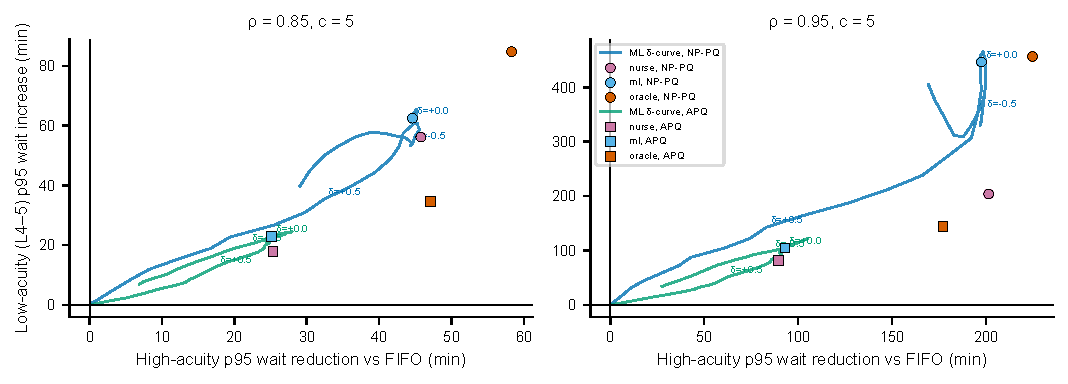
\includegraphics[width=\textwidth]{figures/F5_tradeoff.pdf}
\caption{High-acuity p95 reduction vs.\ low-acuity p95 increase relative to FIFO,
$c=5$, at $\rho=0.85$ and $0.95$: ML $\delta$-curve (lines), nurse, ML ($\delta=0$) and
oracle points, for NP-PQ (circles) and APQ (squares).}
\label{fig:tradeoff}
\end{figure*}

% ============================================================================
\section{Discussion and Limitations}

For ED managers the results reduce to three rules. (i) Judge a triage classifier on tail
waits and on low-acuity harm, not on mean wait or target compliance. (ii) Below about
80\% utilisation almost any informative classifier beats FIFO on high-acuity tails; above it
the bar rises with load, and the relevant quantity is how often high-acuity patients are
sent to the bottom two levels, which should stay well under the $\mathrm{SU}^*$ in
Table~\ref{tab:lookup}. (iii) At high load, pair triage with APQ and choose the ML
threshold by the queue-aware $\delta$, not by accuracy or QWK. Against the planning
hypotheses, the load dependence of the tail bar is confirmed but its magnitude is modest
($J^*\le0.25$), undertriage bias shifts it only slightly, and APQ both lowers the bar and
reduces harm.

The study has limits. rESI-O is an outcome-based proxy, not ground truth: NHAMCS does
not record medication route, so parenteral drugs are not counted as resources, and its
outcome-defined level 2 (2.7\% of visits) is much narrower than the nurses' (14\%), which
inflates apparent nurse overtriage. Errors are assumed independent of load and of other
patients; arrivals are stationary Poisson; there is no abandonment, re-triage or
deterioration while waiting; and service is a single provider stage. Classifier training
ignores survey weights, and NHAMCS immediacy levels are not a uniform ESI. Finally, the
break-even surfaces are specific to the ordered-probit error family; for real classifiers
we recommend the plug-in simulation, which our code supports directly.

\section{Conclusion}
The accuracy an ML triage tool needs depends on the metric and on the load. For mean wait
the bar is trivial at every load; for high-acuity tail waits it rises with utilisation but
stays well below what nurse and ML triage achieve on NHAMCS data, because real errors are
adjacent. The meaningful differences between triagers lie in the harm to low-acuity
patients, where accumulating priority and queue-aware thresholds help most.
Code and results: \todo{repository URL}.

\bibliographystyle{IEEEtran}
\bibliography{refs}

\end{document}
